% !TeX spellcheck = en_EN-English
\documentclass[a4paper]{article}
\usepackage[english]{babel}
\usepackage[utf8]{inputenc}
\usepackage[T1]{fontenc}
\usepackage{a4wide}
\usepackage{amsmath}
\usepackage{amsfonts}
\usepackage{amssymb}
\usepackage{mathrsfs}
\usepackage[small,bf]{caption}
\usepackage{subcaption}
\usepackage{xcolor}
\usepackage{graphicx}
\usepackage{enumerate}
\usepackage{hyperref}
\usepackage{tikz}

\let\origfontsize\fontsize
\def\fontsize#1#2{\origfontsize{11}{14.5}}

\xdef\mypath{C:/Users/majko/Desktop/weather_prediction/images}

\pagestyle{empty}
\setlength{\parindent}{0pt}

\newenvironment{modenumerate}
{\enumerate\setupmodenumerate}
{\endenumerate}

\newif\ifmoditem
\newcommand{\setupmodenumerate}{%
	\global\moditemfalse
	\let\origmakelabel\makelabel
	\def\moditem##1{\global\moditemtrue\def\mesymbol{##1}\item}%
	\def\makelabel##1{%
		\origmakelabel{##1\ifmoditem\rlap{\mesymbol}\fi\enspace}%
		\global\moditemfalse}%
}

\renewcommand{\thesubsection}{\alph{subsection})}

\makeatletter
\def\@seccntformat#1{%
	\expandafter\ifx\csname c@#1\endcsname\c@section\else
	\csname the#1\endcsname\quad
	\fi}
\makeatother
\def\checkmark{\tikz\fill[scale=0.4](0,.35) -- (.25,0) -- (1,.7) -- (.25,.15) -- cycle;} 
\begin{document} 
	
	\pagenumbering{arabic}
	\pagestyle{plain}
	
	\begin{center}
		\sc\large
		ML Project
		\\
		Determining whether weather is good for picnic 
	\end{center}
	
	Author: Marián Kravec

	\section{Data}
	
	\subsection{Source and content}
	Data used for classification and prediction are from Kaggle (\url{https://www.kaggle.com/datasets/sujaykapadnis/whether-prediction-dataset?select=weather_prediction_dataset.csv}).
	\\
	
	Dataset contains weather information from 18 different European cities (or places) measured between years 2000 and 2010 (3654 rows).
	\\
	
	We will use data for 16 of these cities. We will not use data for Roma because it's missing picnic weather label and data for Malmo because it contains only 6 out of 12 columns.
	\\
	
	We have these columns for specific cities:
	
	
	\begin{table}[!h]
		\scalebox{0.7}{
		\begin{tabular}{|p{0.12\textwidth}|p{0.055\textwidth}|p{0.06\textwidth}|p{0.05\textwidth}|p{0.09\textwidth}|p{0.08\textwidth}|p{0.095\textwidth}|p{0.13\textwidth}|p{0.085\textwidth}|p{0.06\textwidth}|p{0.06\textwidth}|p{0.06\textwidth}|p{0.09\textwidth}|}
			\hline
			&  cloud cover & wind speed & wind gust & humidity & pressure & global radiation & precipitation & sunshine & temp mean & temp min & temp max & picnic weather \\ \hline
			De Bilt & \checkmark & \checkmark & \checkmark & \checkmark & \checkmark & \checkmark & \checkmark & \checkmark & \checkmark & \checkmark & \checkmark & \checkmark \\ \hline
			Tour &  & \checkmark &  & \checkmark & \checkmark & \checkmark & \checkmark &  & \checkmark & \checkmark & \checkmark & \checkmark \\ \hline
			Ljubljana & \checkmark & \checkmark &  &  & \checkmark & \checkmark & \checkmark & \checkmark & \checkmark & \checkmark & \checkmark & \checkmark \\ \hline
			Maastricht & \checkmark & \checkmark & \checkmark & \checkmark & \checkmark & \checkmark & \checkmark & \checkmark & \checkmark & \checkmark & \checkmark & \checkmark \\ \hline
			Muenchen & \checkmark & \checkmark & \checkmark & \checkmark & \checkmark & \checkmark & \checkmark & \checkmark & \checkmark & \checkmark & \checkmark & \checkmark \\ \hline
			Perpignan &  & \checkmark &  & \checkmark & \checkmark & \checkmark & \checkmark &  & \checkmark & \checkmark & \checkmark & \checkmark \\ \hline
			Heathrow & \checkmark &  &  & \checkmark &  & \checkmark & \checkmark & \checkmark &  & \checkmark & \checkmark & \checkmark \\ \hline
			Budapest & \checkmark &  &  & \checkmark & \checkmark & \checkmark & \checkmark & \checkmark & \checkmark & \checkmark & \checkmark & \checkmark \\ \hline
			Montelimar &  & \checkmark &  & \checkmark & \checkmark & \checkmark & \checkmark &  & \checkmark & \checkmark & \checkmark & \checkmark \\ \hline
			Dusseldorf & \checkmark & \checkmark & \checkmark & \checkmark & \checkmark & \checkmark & \checkmark & \checkmark & \checkmark & \checkmark & \checkmark & \checkmark \\ \hline
			Dresden & \checkmark & \checkmark & \checkmark & \checkmark &  & \checkmark & \checkmark & \checkmark & \checkmark & \checkmark & \checkmark & \checkmark \\ \hline
			Stockholm & \checkmark &  &  &  & \checkmark &  & \checkmark & \checkmark & \checkmark & \checkmark & \checkmark & \checkmark \\ \hline
			Sonnblick & \checkmark &  &  & \checkmark &  & \checkmark & \checkmark & \checkmark & \checkmark & \checkmark & \checkmark & \checkmark \\ \hline
			Basel & \checkmark &  &  & \checkmark & \checkmark & \checkmark & \checkmark & \checkmark & \checkmark & \checkmark & \checkmark & \checkmark \\ \hline
			Kassel &  & \checkmark & \checkmark & \checkmark & \checkmark & \checkmark & \checkmark & \checkmark & \checkmark & \checkmark & \checkmark & \checkmark \\ \hline
			Oslo & \checkmark & \checkmark & \checkmark & \checkmark & \checkmark & \checkmark & \checkmark & \checkmark & \checkmark & \checkmark & \checkmark & \checkmark \\ \hline
		\end{tabular}
		}
	\end{table}

	\subsection{Data preparation}
	
	Firstly we need to prepare data into suitable form for models. We split data into city specific dataset. 
	\\
	
	Then when we are preparing data for model we load data for required city (or multiple cities) and shuffle rows. Then we split data firstly into variables and labels (meaning column-wise) and secondly into train, test and validation parts (meaning row-wise). Finally for train data we compute average and variance of each column to normalize all three datasets using these values.
	
	\newpage

	\section{SVC comparison}
	
	We will try to classify whether weather is suitable for picnic in Basel. We will train three Support vector classifiers to compare their results.
	\\
	
	We will train these three models:
	\begin{itemize}
		\item C-Support Vector Classifier (sklearn.svm.SVC) with radial basis function kernel (we will optimize regularization parameter C)
		\item Linear Support Vector Classifier (sklearn.svm.LinearSVC) (we will optimize regularization parameter C)
		\item Linear SVC with SGD (stochastic gradient descend) training (sklearn.linear\_model.SGDClassifier with loss parameter "hinge") (we will optimize constant that multiplies the regularization term $\alpha$)
	\end{itemize}

	As a score for each model we will take percentage of correctly assigned labels. To make this value more informative we will use cross validation and final score would be average score of 5-fold cross validation.
	
	After training (and optimizing chosen parameters) we get these test scores:
	
		\begin{table}[!h]
			\begin{tabular}{|l|l|l|l|}
				\hline
				model & optimized parameter & parameter value & test score  \\ \hline
				RBF kernel SVC & C & 23 & 0.89315 \\ \hline
				Linear SVC & C & 23 & 0.94247 \\ \hline
				Linear SVC with SGD& $\alpha$ & $10^{-8}$ & 0.89315 \\ \hline
			\end{tabular}
	\end{table} 

	Based on this information it seems like Linear SVC without SGD is better then other two models which seems to equally good. However as Goodhart's law says "When a measure becomes a target, it ceases to be a good measure" which means that test score is not good measure for our models (test dataset was used to choose best parameter value). 
	\\
	
	If we compute validation score for each of these models:
	
	\begin{table}[!h]
		\begin{tabular}{|l|l|}
			\hline
			model &  validation score  \\ \hline
			RBF kernel SVC & 0.92632 \\ \hline
			Linear SVC & 0.95361 \\ \hline
			Linear SVC with SGD &  0.88804 \\ \hline
		\end{tabular}
	\end{table} 

	We can see that Linear SVC still has best score, so we can consider it to be best model out of these three. We can also see that based on validation score it seems like SVC with RBF kernel is better model than Linear SVC with SGD. 
	
	\newpage

	\section{Basic neural network versus transfer learning}
	
	We have 5 cities for which we have all 12 columns, those cities are: De Bilt, Maastrich, Muenchen, Dusseldorf, Oslo. What we will try to do is train standard sequential neural network to classify whether weather in Maastrich is good for picnic. 
	\\
	
	We will compare two neural network. First NN will be trained solely using data from Masstrich. Second will be firstly trained on data from four other cities then all layers except last one will be frozen and last layer would be retrained using Masstrich data. We will then compare those two networks.  
	\\
	
	We tried multiple neural networks with different number of layers and different number of neurons in each layer and finally we ended sequential neural network with four dense layers. First three of these use hyperbolic tangent as activation function and have 24, 8 and 12 neurons respectively. Last layer use softmax as activation function and contain 2 neurons representing true and false values of our labels.    
	\\
	
	Now we can take look at accuracy of our three models (we consider model we pre-trained to use for transfer learning as third model). In this case test accuracy is computed during training by Keras library itself using 10\% of provided data which means that test accuracy of model used as pre-trained model is not accuracy on Masstrich data but accuracy on provided data from four other cities.
	
	
	\begin{figure}[h!]
		\centerline{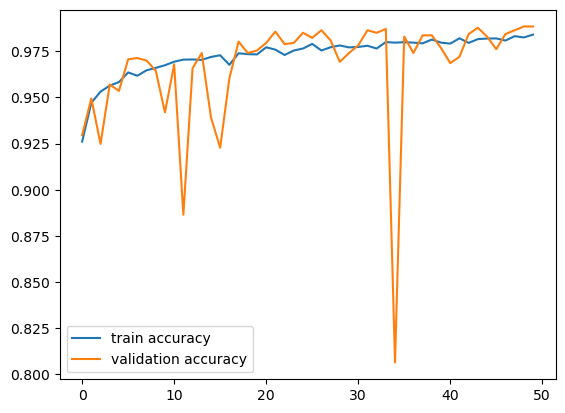
\includegraphics[width=0.85\textwidth]{\mypath/accuracy_pretrain.png}}
		\caption{Accuracy of model used for transfer learning during training}
	\end{figure}

	\begin{figure}[h!]
		\centerline{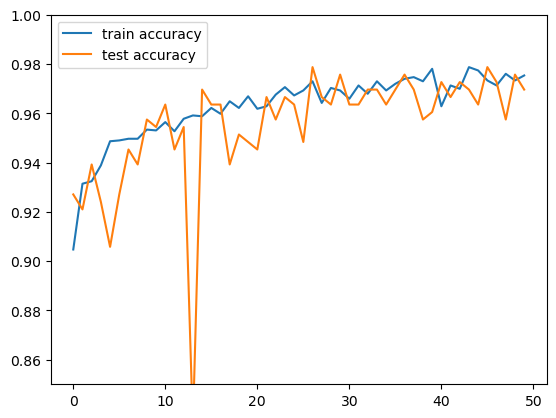
\includegraphics[width=0.85\textwidth]{\mypath/accuracy_basic.png}}
		\caption{Accuracy of model trained using only Masstrich data}
	\end{figure}

	\begin{figure}[h!]
		\centerline{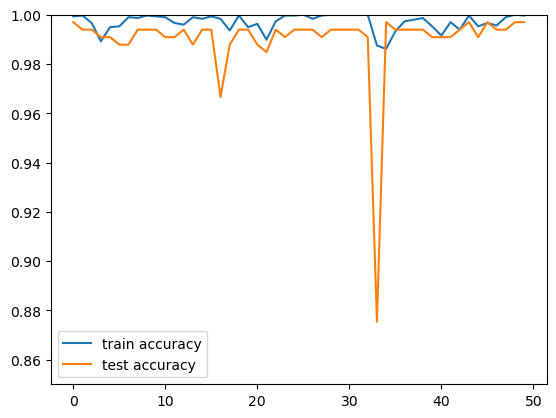
\includegraphics[width=0.85\textwidth]{\mypath/accuracy_transfer.png}}
		\caption{Accuracy of model trained using Masstrich data and pre-trained model}
	\end{figure}

	
	
	\begin{table}[!h]
		\begin{tabular}{|l|l|}
			\hline
			model &  validation accuracy  \\ \hline
			Pre-trained on different cities  & 0.98356 \\ \hline
			Standard Neural Network & 0.97260 \\ \hline
			Trasfer learning using pre-trained &  0.99178 \\ \hline
		\end{tabular}
	\end{table} 
\end{document}